
%%%%%%%%%%%%%%%% Nm Tutorial %%%%%%%%%%%%%%%%%%%%
\chapter{Netzwerk-Management Anleitung}
\label{sec:nm_tutorial}
Diese Anleitung basiert auf dem entsprechenden AUTOSAR Workshop von Elektrobit vom 11.12.2012 und wurde an einigen Stellen gekürzt und erweitert. \\

\begin{compactitem}
    \item Module importieren (CanNm, CanSM, ComM, Nm)
    \item System Description und DBC anpassen
    \begin{compactitem}
        \item Service Ports einrichten
        \item NM Botschaften erstellen und Nodes zuordnen
        \item ARXML und DBC importieren
        \item Wizard "`Calculate Handle IDs"' ausführen
        \item Wizard "`Calculate Derivable Values"' ausführen
    \end{compactitem}
    \item ComM
    \begin{compactitem}
        \item ./General/Enable Rte Usage: True
        \item ./Optimization/Network Start Indication Failure: DISABLE
        \item ./Users/: Add User
        \item ./Network Channel/: Channel hinzufügen
        \begin{compactitem}
            \item Main Function Period: 0.01
            \item User Per Channel: User inzufügen
        \end{compactitem}
    \end{compactitem}
    \item Nm
    \begin{compactitem}
        \item Number of Nm Channels: 1
        \item ./List of Nm Channels/: Channel hinzufügen und ComM Channel Reference setzen
    \end{compactitem}
    \item CanIf
    \begin{compactitem}
        \item ./CanIfInitConfiguration/CanIfTxPduConfig/: NM PDU auswählen
        \item CanIfTxUserType: CAN\_NM
        \item CanIfRxUserType: CAN\_NM
    \end{compactitem}
    \item CanNM
    \begin{compactitem}
        \item ./CanNmGlobalConfig/Optimization/
        \begin{compactitem}
            \item CanNm Network Timeout: DISABLE
            \item CanIf Transmission Error: DISABLE
        \end{compactitem}
        \item ./CanNmGlobalConfig/Channel Configuration/: Channel hinzufügen
        \begin{compactitem}
            \item NM Channel Reference: Vorher erstellter
            \item Main Funtion Period: 0.01
            \item PDU Length: 0
            \item Node Identifier Position: CANNM\_PDU\_OFF (CANNM\_PDU\_BYTE0 für NM-High)
            \item Control Bit Vector Position: CANNM\_PDU\_OFF
            \item PDU User Data Length: 0 (6 bei NM-High)
            \item Message Cycle Time: 0.5
            \item Message Cycle Offset: 0
            \item Messag Timeout Time: 4
            \item Timeout Time: 1
            \item Wait Bus Sleep Time: 4
            \item Repeat Message Time: 0.5
            \item Transmit PDU Referece: NM PDU
        \end{compactitem}
    \end{compactitem}
    \item CanSM
    \begin{compactitem}
        \item ./List of Configurations/: Config hinzufügen und öffnen
        \item ./List of Can Networks/: Hinzufügen und öffnen
        \item ComM Channel: Vorher ersteller
        \item Com Rx PDU Group: RXPDUS\_GLOBAL
        \item Com Tx PDU Group: TXPDUS\_GLOBAL
        \item Can Controller hinzufügen und Can Config auswählen
    \end{compactitem}





    \item SchMMainFunctionMapping
    \begin{compactitem}
        \item SchMMappedToTask immer auf zyklische OS Task setzen
        \item CanSM Main Function hinzufügen
        \begin{compactitem}
            \item SchMMainFunctionRef: CanSM\_MainFunction
            \item SchMMainFunctionHeader: CanSM\_SchM.h
        \end{compactitem}
        \item ComM Main Function hinzufügen
        \begin{compactitem}
            \item SchMMainFunctionRef: ComM\_MainFunction\_0
            \item SchMMainFunctionHeader: ComM.h
        \end{compactitem}
        \item CanNM Main Function hinzufügen
        \begin{compactitem}
            \item SchMMainFunctionRef: CanNm\_MainFunction\_0
            \item SchMMainFunctionHeader: CanNM.h
        \end{compactitem}
    \end{compactitem}

    \item SchMModuleConfiguration
    \begin{compactitem}
        \item CanNm Konfiguration hinzufügen
        \begin{compactitem}
            \item SchMModuleLiteral: CanNm
            \item SchMUseInstanceId: False
            \item InstanceConfiguration hinzufügen
            \item SchMInstanceId: 0
            \item SchMInstanceLiteral: SCHM\_CANNM\_INSTANCE\_0
            \item ExcelusiveAreaConf hinzufügen
            \item SchmExclusiveAreaId: 0
            \item SchMExclusiveAreaLiteral: SCHM\_CANNM\_EXCLUSIVE\_AREA\_0
            \item SchMExclusiveAreaType: EB\_FAST\_LOCK
        \end{compactitem}
        \item ComM Konfiguration hinzufügen
        \begin{compactitem}
            \item SchMModuleLiteral: ComM
            \item SchMUseInstanceId: False
            \item InstanceConfiguration hinzufügen
            \item SchMInstanceId: 0
            \item SchMInstanceLiteral: SCHM\_COMM\_INSTANCE\_0
            \item ExcelusiveAreaConf hinzufügen
            \item SchmExclusiveAreaId: 0
            \item SchMExclusiveAreaLiteral: SCHM\_COMM\_EXCLUSIVE\_AREA\_0
            \item SchMExclusiveAreaType: EB\_FAST\_LOCK
        \end{compactitem}
    \end{compactitem}



    \item EcuM
    \begin{compactitem}
        \item ./Configuration/Init List Two/
        \begin{compactitem}
            \item Element hinzufügen
            \item ModuleID: CanSM
            \item ModuleService: Init
            \item Element hinzufügen
            \item ModuleID: CanNm
            \item ModuleService: Init
            \item Module Config String: \&CanNmGlobalConfig
            \item Element hinzufügen
            \item ModuleID: Nm
            \item ModuleService: Init
            \item Module Config String: ((void*)-1)
        \end{compactitem}
        \item ./Configuration/Init List Three/
        \begin{compactitem}
            \item Element hinzufügen
            \item ModuleID: ComM
            \item ModuleService: Init
        \end{compactitem}
    \end{compactitem}
    \item Rte
    \begin{compactitem}
        \item Service Port Mapping: Service Port Generation
        \item SWC\_XX/UserRequest mit ComM/UR\_ComMUser\_0 verbinden
        \item SWC\_XX/CurrentMode mit ComM/UM\_ComMUser\_0 verbinden
    \end{compactitem}
    \item Implementation
    \begin{compactitem}
        \item Rte\_Call\_UserRequest\_RequestComMode(FULL\_COMMUNICATION)
        \item Rte\_Call\_UserRequest\_RequestComMode(NO\_COMMUNICATION)
    \end{compactitem}





\end{compactitem}
























%%%%%%%%%%%%%%%% VCAN-API %%%%%%%%%%%%%%%%%%%%
\chapter{VCAN-API}
\label{sec:vcan_api}
Dieses Kapitel beschreibt die im Laufe des Projektes erstellte Software zur Kommunikation per virtuellem CAN. Alle Informationen über das Protokoll wurden per Reverse Engineering ermittelt.

\section{Protokoll}
\label{sec:vcan_protokoll}
Das VCAN-Protokoll besteht aus einem Binär-Format, dass per TCP-Socket übertragen wird. Der Aufbau und Abbau der TCP-Verbindungen wird verwendet um Clients am Gateway an- und abzumelden. Zudem müssen Socket-Fehler abgefangen werden, da ein ordnungsgemäßer Verbindungsabbau nicht gegeben sein muss.

\begin{figure}[ht]
\centering
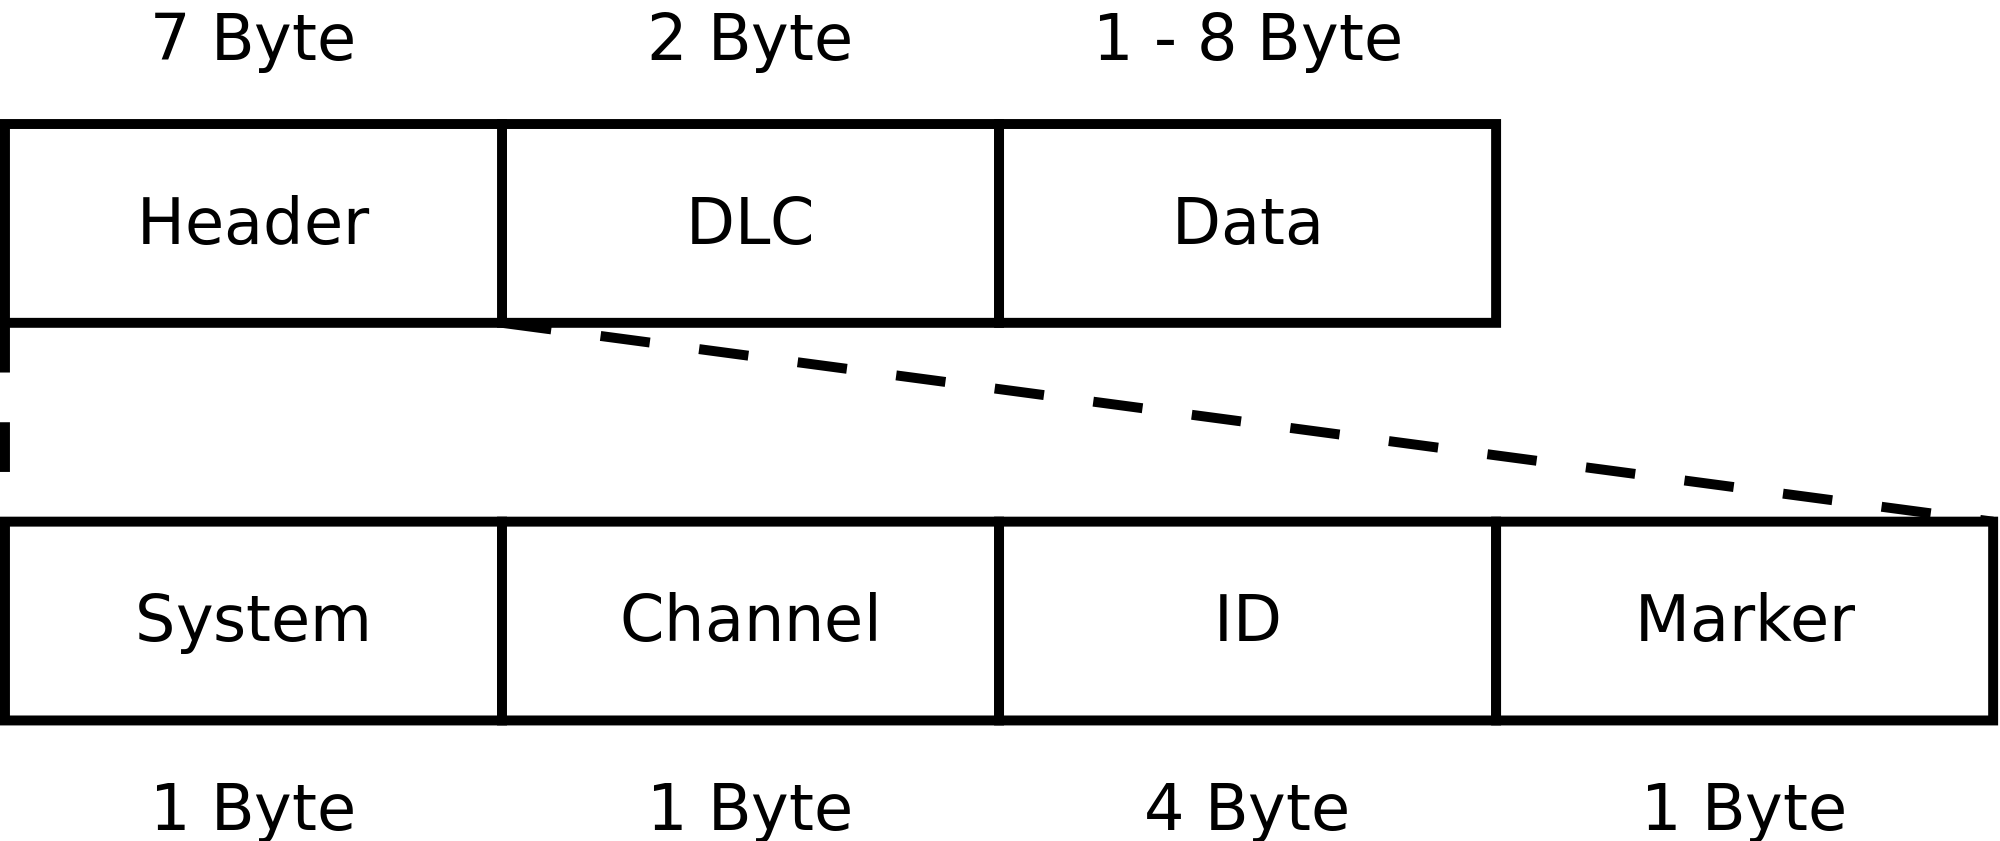
\includegraphics[width=0.8\textwidth]{vcan_protokoll}
\caption{Überblick über das VCAN Protkoll}
\label{fig:vcan_protokoll}
\end{figure}

Das eigentliche Binär-Format des Protokolls ist in Abbildung \ref{fig:vcan_protokoll} zu sehen. Das Format besteht aus einem Header, dem DLC-Feld und den eigentlichen Daten. Der Header enthält unter anderem die ID der Botschaft. Die Nutzdaten können 1 bis 8 Byte lang sein. Im folgenden ist eine ausfürliche Auflistung der Felder dargestellt. Die Byte-Reheinfolge entspricht Big-Endian. Tabelle \ref{tab:vcanbotschaft} zeigt eine Beispiel-Botschaft ohne TCP- und Ethernet-Header.

\begin{description}
    \item[System] \hfill \\ Angabe eines Systems (zum Beispiel CAN oder LIN). Eine Auflistung der möglichen Werte ist in Tabelle \ref{tab:vcansysteme} zu finden. Die symbolischen Namen stammen dabei aus dem Elektrobit Gateway. Höhere Werte führen beim EB Gateway zu Fehlern beziehungsweise Abstürzen.
    \item[Channel] \hfill \\ Enthält eine Kanal-Nummer. Kann Werte von 0 bis 255 annehmen.
    \item[ID] \hfill \\ CAN-ID der Botschaft.
    \item[Marker] \hfill \\ Markiert extended CAN Frames. 0 steht für einen standard frame, jeder andere Wert für ein extendend Frame. Dies Byte könnte weitere Funktionalität bei LIN oder FlexRay Systemen haben.
    \item[DLC] \hfill \\ Anzahl der Daten-Bytes. Kann bei CAN nur Werte von 1 bis 8 annehmen. 
    \item[Data] \hfill \\ Nutzdaten. Die Anzahl der Bytes entspricht dem Wert im DLC-Feld.
\end{description}

\begin{table}[ht]
    \centering
    \begin{minipage}{0.45\textwidth}		
        \begin{tabular}[h]{c l}
            Hex Wert & Symbolischer Name \\
            \toprule
            0 & Unknown\\
            1 & Flexray1\\
            2 & Flexray2\\
            3 & CAN1\\
            4 & CAN2\\
            5 & CAN3\\
            6 & CAN4\\
            7 & LIN1\\
            8 & LIN2\\
            9 & bad allocation\\
            a & æI@\\
            b & <null>\\
            c & Fehler\\
            d & Fehler\\
            \dots & \dots\\
            \bottomrule
        \end{tabular}
        \caption{Liste der VCAN Systeme}
        \label{tab:vcansysteme}
    \end{minipage}\hfill
    \begin{minipage}{0.45\textwidth}
        \begin{tabular}[h]{c l}
            Hex Wert & Bedeutung \\
            \toprule
            03 & System: CAN1\\
            \midrule
            00 & Channel: 0\\
            \midrule
            42 & \multirow{4}{*}{CAN-ID (hex): 742}\\
            07 & \\
            00 & \\
            00 & \\
            \midrule
            00 & Standard Frame\\
            \midrule
            04 & \multirow{2}{*}{DLC: 4 Bytes}\\
            00 & \\
            \midrule
            00 & \multirow{4}{*}{Daten: 00:00:2A:00}\\
            00 & \\
            2a & \\
            00 & \\
            \bottomrule
        \end{tabular}
        \caption{Beispiel VCAN Botschaft}
        \label{tab:vcanbotschaft}
    \end{minipage}
\end{table}

Das Protokoll, wie es im Elektrobit-Gateway eingesetzt wird, hat einige Besonderheiten. So werden gelegentlich die Daten-Bytes mehrerer Botschaften angehängt. Hierbei wird der Header nur einmal, jedoch die Daten mehrerer Botschaften übermittelt. Auch wird zeitweise der Daten-Bereich einer Botschaft mehrfach angehängt. Das Verhalten konnte nicht zuverlässig nachvollzogen werden. Es hat jedoch den Anschein, dass diese Probleme durch eine hohe Netzwerk-Last beziehungsweise -Latenz hervorgerufen werden. Da nicht eindeutig eine Mehrfachsendung einer Botschaft von verschiedene Botschaften in einem Paket unterschieden werden kann, wurde dieses Verhalten nicht implementiert. 


\section{Projekt Struktur}
\label{sec:vcan_struktur}
Im Folgenden wird die Dateistruktur des Projektes näher betrachtet. Abbildung \ref{fig:vcan_api_uml} zeigt ein UML-Klassendiagramm der VCAN-API.

Die reine VCAN-API besitzt als Abhängigkeit lediglich Module der \emph{CPython} Standardbibliothek. Andere Python Interpreter wie Jython werden zur Zeit nicht unterstützt. Support für PCAN ist nur unter Windows verfügbar und benötigt die PCAN-Basic-API.

Die vom Gateway und der VCAN-Applikation genutzte grafischen Oberfläche basiert auf \emph{wxPython}\footnote{\url{http://www.wxpython.org/}}. Der Benchmark benötigt das Modul \emph{pygame}\footnote{\url{http://www.pygame.org/}} für konstante Timer und \emph{rpy}\footnote{\url{http://rpy.sourceforge.net/}} für die Auswertung der Ergebnisse mittels \emph{R}\footnote{\url{http://www.r-project.org/}}.

\begin{figure}[ht]
\centering
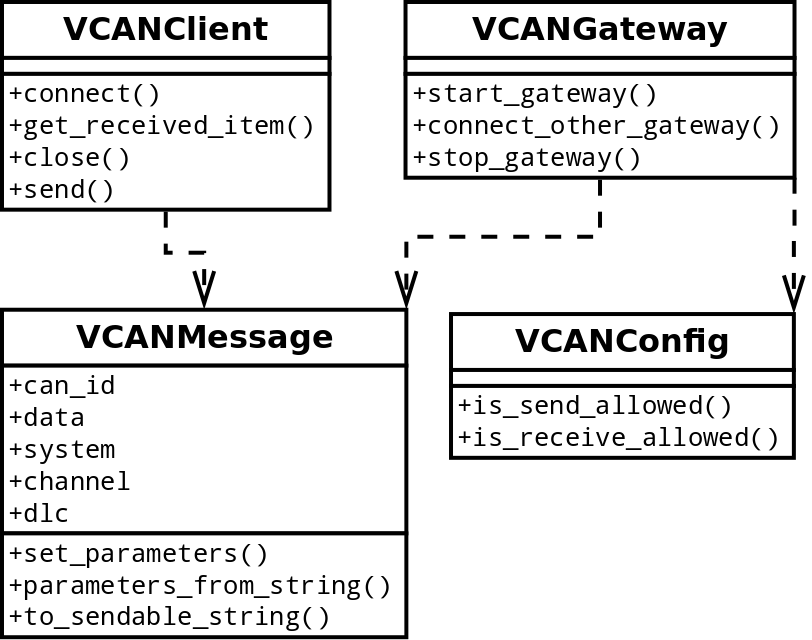
\includegraphics[width=0.8\textwidth]{vcan_api_uml}
\caption{UML-Klassendiagramm der VCAN-API}
\label{fig:vcan_api_uml}
\end{figure}

\begin{description}
    \apiitem{./vcan\_api/}
    Dieses Verzeichnis enthält die gesamte VCAN-API.
    \begin{description}
        \apiitem{./vcan\_api/\_\_init\_\_.py}
        VCAN-API Python Pyackage.
        \apiitem{./vcan\_api/PCANBasic.py}
        API zur Nutzung des PEAK-PCAN-USB-Adapters. Diese Datei stammt von PEAK.
        \apiitem{./vcan\_api/vcan\_client.py}
        Enthält die Klasse VCANClient.
        \apiitem{./vcan\_api/vcan\_config.py}
        Enthält die Klasse VCANConfig.
        \apiitem{./vcan\_api/vcan\_config.xsd}
        XML-Schema für Firewall-Konfigurationen.
        \apiitem{./vcan\_api/vcan\_exception.py}
        Enthält die Klasse VCANException.
        \apiitem{./vcan\_api/vcan\_gateway.py}
        Enthält die Klasse VCANGateway.
        \apiitem{./vcan\_api/vcan\_message.py}
        Enthält die Klasse VCANMessage und einige Konstanten um diese zu Nutzen.
    \end{description}
    \apiitem{./example\_client.py}
    Verschiedene Beispiele für die Implementierung eines VCAN-Clients.
    \apiitem{./example\_gateway.py}
    Verschiedene Beispiele für die Implementierung eines VCAN-Gateways.
    \apiitem{./gateway.py}
    Ein simples Gateway mit grafischer Oberfläche.
    \apiitem{./gateway\_rules.xml}
    Eine Beispiel-Konfiguration der im Gateway eingebauten Firewall-Regeln.
    \apiitem{./vcan\_app.py}
    VCAN Applikation um den Scheinwerfer-Versuchsaufbau anzusteuern.
\end{description}


\section{Gateway API}
\label{sec:vcan_gateway_api}

% class VCANGateway
\begin{description}
    \apiitem{class VCANGateway(receive\_callback=None, connection\_callback=None)}
    Das Gateway nimmt Verbindungen von Clients entgegen und verteilt eingehende Botschaften an alle angemeldeten Clients weiter.
    \begin{description}
        \apiitem{start\_gateway(host='127.0.0.1', port=10020, rulesfile='')}
        Startet das Gateway auf IP \texttt{host} und dem Port \texttt{port}. Auf dem ausführenden Rechner muss ein Netzwerk-Interface mit der entsprechenden IP existieren. Der Port darf nicht durch eine andere Anwendung belegt sein. Optional kann eine Regeldatei angegeben werden um Firewall-Regeln zu definieren. Dies ist noch experimentell.
        \apiitem{stop\_gateway()}
        Stoppt das Gateway wieder. Anschließend kann mittels der \texttt{start\_gateway} Methode wieder gestartet werden. Es werden jedoch alle Verbindungen getrennt, und die Host IP muss ein weiteres mal angegeben werden.
        \apiitem{connect\_other\_gateway(host, port=10020)}
        Ein Gateway kann sich zu einem anderen Gateway verbinden um ein Netz zu bilden. Das Ziel-Gateway muss unter der IP \texttt{host} und dem Port \texttt{port} erreichbar sein. Diese Methode ist hilfreich, wenn zum Beispiel eine Firewall eingehende Verbindungen verbietet oder ein Gateway unter Linux mit einem Windows-Gateway verbunden wird, um den PCAN nutzen zu können.
        \apiitem{pcan\_init()}
        Initialisiert den ersten gefundenen PEAK-PCAN USB-Dongle mit einer Baud-Rate von 500kbaud. Das gwählte USB-Interface und die Baud-Rate können zur Zeit nur im Code geändert werden. PCAN Support ist im Moment nur unter Windows vorhanden und wird ansonsten durch eine VCANException markiert.
        \apiitem{pcan\_uninit()}
        Deinitialisiert den PEAK-PCAN USB-Dongle.
    \end{description}
\end{description}

% class VCANConfig
\begin{description}
    \apiitem{class VCANConfig(rulesfile)}
    Diese Klasse wird verwendet um Firewall-Regeln im Gateway zu implementieren. Hierzu wird eine XML-Datei mit Regeln übergeben. Diese Datei muss dem beiligenden Schema \texttt{vcan\_config.xsd} entsprechen. Das Gateway ist dafür verantwortlich die entsprechenden Überprüfungen beim Senden und Empfangen durchzuführen.
    \begin{description}
        \apiitem{is\_send\_allowed(ip, can\_id)}
        Überprüft ob die IP \texttt{ip} eine Botschaft mit der ID \texttt{can\_id} senden darf. Gibt True zurück falls erlaubt, und False falls verboten.
        \apiitem{is\_receive\_allowed(ip, can\_id)}
        Überprüft ob die IP \texttt{ip} eine Botschaft mit der ID \texttt{can\_id} empfangen darf. Gibt True zurück falls erlaubt, und False falls verboten.
    \end{description}
\end{description}

% class VCANException
\begin{description}
    \apiitem{class VCANException(value)}
    Exception der VCAN-API. Wird beim Gateway verwendet, falls die PCAN-Verbindung nicht initialisiert werden kann.
\end{description}




\section{Client API}
\label{sec:vcan_client_api}

% class VCANClient
\begin{description}
    \apiitem{class VCANClient(q\_length=1024)}
    Diese Klasse kann verwendet werden, um Zugriff auf den VCAN zu erhalten. Es bietet Funktionen um eine Verbindung aufzubauen und zu schließen. Außerdem können Botschaften empfangen und gesendet werden. Standardmäßig erfolgt das Empfangen auf Polling-Basis. Hierzu wird eine Queue der Länge \texttt{q\_length} angelegt. Der Anwender ist verantwortlich die eingehenden Daten häufig genug zu pollen. Alternativ kann für das Empfangen eine Callback-Funtion angegeben werden.
    \begin{description}
        \apiitem{connect(ip, port=10020, receive\_data=True, callback=None)}
        Verbindet den Client mit einem Gateway auf IP \texttt{ip} und Port \texttt{port}. Über den Schalter \texttt{receive\_data} kann das Empfangen von Botschaften deaktiviert werden. Der Parameter \texttt{callback} kann verwendent werden um eine Funktions-Referenz zu übergeben, die empfangene Botschaften direkt verarbeitet. Wirft \texttt{VCANException} falls keine Verbindung hergestellt werden kann.
        \apiitem{close(sleep\_time=0.5)}
        Schließt die aktuelle Verbindung. Der Parameter \texttt{sleep\_time} wird verwendet um nach dem Schließen der Verbindung einen Moment zu warten. Damit werden Eigenheiten des EB-Gateways und der AUTOSAR-Anwendungen ausgeglichen, da es ansonsten zu Fehlern kommen kann. Die Angabe erfolgt in Sekunden.
        \apiitem{get\_received\_item()}
        Gibt die älteste empfangene Botschaft zurück. Falls die Queue leer ist wird \texttt{None} zurückgegeben. Diese Methode muss im Polling-Betrieb häufig genug aufgerufen werden, um Daten-Verlust zu vermeiden.
        \apiitem{send(message, sleep\_time=0.2)}
        Sende die Botschaft \texttt{message} zum verbundenden Gateway. Die Botschaft kann sowohl als Binär-String, als auch als VCANMessage vorliegen. Der Parameter \texttt{sleep\_time} wird verwendet um Fehler zu vermeiden indem nach dem Senden ein Moment gewartet wird. Falls nur Applikation angebunden sind, die die VCAN-API nutzen kann dieser Wert auf 0 gesetzt werden. AUTOSAR-Applikation haben jedoch Probleme mit zu geringen Warte-Zeiten und können Botschaften verlieren oder sogar abstürzen. Die Angabe erfolgt in Sekunden. Falls der Client zu keinem Gateway verbunden ist, wird eine \texttt{VCANException} geworfer.
    \end{description}
\end{description}

% class VCANMessage
\begin{description}
    \apiitem{class VCANMessage()}
    Repräsentiert eine Botschaft in der VCAN-API. Der Konstruktur generiert eine leere Botschaft. Diese kann entweder über \texttt{set\_parameters()} von Hand mit Parametern gefüllt werden, oder über \texttt{parameters\_from\_string()} von einer eingehenden Nachricht aus einem Binär-String.
    \begin{description}
        \apiitem{set\_parameters(can\_id,  data, system, channel, dlc=None)}
        Setzt die Parameter der Nachricht entsprechend den Parametern. Parameter \texttt{can\_id} gibt die ID der Botschaft an. Die Nutzdaten sind werden in \texttt{data} erwartet und müssen als Liste übergeben werden. Die Parameter \texttt{system} und \texttt{channel} geben das entsprechende System und den Kanal an. Standard-Werte sind CAN und Kanal 0. Weitere Möglichkeiten sind in der Datei \texttt{vcan\_message.py} als Konstanten hinterlegt. Der letzte Parameter, \texttt{dlc}, gibt die Länge der Daten an. Falls \texttt{None} übergeben wird, wird die Länge des Daten-Arrays verwendet.
        \apiitem{parameters\_from\_string(m\_string)}
        Setzt die Parameter der Nachricht anhand des Binär-Strings \texttt{m\_string}. Diese entsprechen direkt dem TCP-Paket und können hierdurch in eine VCAN-API-konforme Form gebracht werden.
        \apiitem{to\_sendable\_string()}
        Wandelt die Botschaft in einen Binär-String um, der per TCP versendet werden kann.
    \end{description}
\end{description}

% class VCANException
\begin{description}
    \apiitem{class VCANException()}
    Exception der VCAN-API. Wird geworfen falls die Verbindung zu einem Gateway scheitert, oder eine Nachricht gesendet wird obwohl keine Verbindung besteht. Außerdem siehe \ref{sec:vcan_gateway_api}
\end{description}




\section{Beispiel Anwendungen}
\label{sec:vcan_beispiele}
Im Folgenden sind einige Beispiel Anwendungen aufgeführt, die den VCAN nutzen. Da der Quellcode weitreichend selbsterklärend ist, wird auf eine Erläuterung der Beispiele verzichtet.

\subsection{Gateway}
\label{sec:vcan_gateway_beispiele}
\begin{lstlisting}[frame=single, language=Python, basicstyle=\footnotesize, caption={Einfaches Gateway}, label={lst:bsp_gateway1}]
import vcan_api

gw = vcan_api.VCANGateway()
gw.start_gateway(host='127.0.0.1', port=10020)
raw_input("Press key to stop...\n")
gw.stop_gateway()
\end{lstlisting}

\begin{lstlisting}[frame=single, language=Python, basicstyle=\footnotesize, caption={Gateway mit Callbacks}, label={lst:bsp_gateway2}]
import vcan_api

def __message_callback(message):
  print message

def __connection_callback(connection, accepting):
  if accepting == True:
    print "Connection accepted: " + str(connection)
  else:
    print "Connection closed: " + str(connection)

gw = vcan_api.VCANGateway(receive_callback=__message_callback, connection_callback=__connection_callback)
gw.start_gateway(host='127.0.0.1', port=10020)
raw_input("Press key to stop...\n")
gw.stop_gateway()
\end{lstlisting}

\begin{lstlisting}[frame=single, language=Python, basicstyle=\footnotesize, caption={Gateway mit PCAN-Anbindung}, label={lst:bsp_gateway3}]
import vcan_api

gw = vcan_api.VCANGateway()
gw.start_gateway(host='127.0.0.1', port=10020)
gw.pcan_init()
raw_input("Press key to stop...\n")
gw.pcan_uninit()
gw.stop_gateway()
\end{lstlisting}

\begin{lstlisting}[frame=single, language=Python, basicstyle=\footnotesize, caption={Gateway mit Verbindung zu anderem Gateway}, label={lst:bsp_gateway4}]
import vcan_api

gw = vcan_api.VCANGateway()
gw.start_gateway(host='127.0.0.1', port=10020)
try:
  gw.connect_other_gateway('141.41.31.148', port=10020)
except vcan_api.VCANException:
  print "Could not connect to other gateway!"
raw_input("Press key to stop...\n")
gw.stop_gateway()
\end{lstlisting}

\subsection{Client Beispiele}
\label{sec:vcan_client_beispiele}
\begin{lstlisting}[frame=single, language=Python, basicstyle=\footnotesize, caption={Empfangsclient via Callback}, label={lst:bsp_client1}]
import time
import vcan_api

def __receive_message(message):
  m = vcan_api.VCANMessage()
  m.parameters_from_string(message)
  print m

client = vcan_api.VCANClient()
client.connect('127.0.0.1', port=10020, callback=__receive_message)

while True:
  time.sleep(0.5)

client.close()
\end{lstlisting}

\begin{lstlisting}[frame=single, language=Python, basicstyle=\footnotesize, caption={Empfangsclient via Polling}, label={lst:bsp_client2}]
import time
import vcan_api

client = vcan_api.VCANClient()
client.connect('127.0.0.1', port=10020)

while True:
  time.sleep(0.1)
  message = client.get_received_item()
  if message == None:
    continue
  m = vcan_api.VCANMessage()
  m.parameters_from_string(message)
  print m

client.close()
\end{lstlisting}

\begin{lstlisting}[frame=single, language=Python, basicstyle=\footnotesize, caption={Zyklisch sendender Client via Threads}, label={lst:bsp_client3}]
import thread
import time
import vcan_api

def __send(client, value):
  while (True):
    print "sending..."
    data = [0,0,1,value,0,0,0,0]
    m = vcan_api.VCANMessage()
    m.set_parameters(int("3c0", 16),  data)
    sclient.send(m,sleep_time=0.5)

client = vcan_api.VCANClient()
client.connect('127.0.0.1', port=10020)

value = 42
thread.start_new_thread(__send, (client, value,))

raw_input("Press key to exit...\n")
client.close()
\end{lstlisting}









